\subsubsection{漏洞种类及危害}
\textbf{释放后使用(UAF)}:

释放后使用漏洞发生在程序试图使用已释放的内存时。通常,内存释放后,操作系统会将该内存标记为可重新使用,但并不会立即清空其内容。如果程序在内存释放后继续访问该内存,就可能导致安全漏洞。该漏洞的介绍如图\ref{fig:UAF}所示。
	\begin{figure}[htbp]
		\centering
		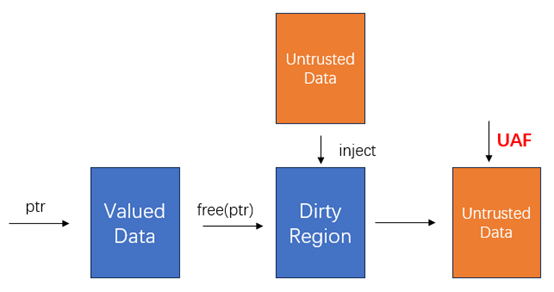
\includegraphics[width=0.5\textwidth]{pictures/UAF.png}
		\caption{释放后使用漏洞图示}
		\label{fig:UAF}
	\end{figure}
攻击者可能利用释放后使用漏洞来执行未经授权的代码,例如通过释放内存但保留对其的引
用,然后在后续代码中使用该引用,从而导致恶意代码执行。同时可能导致程序崩溃或不稳
定,因为操作已释放的内存区域可能导致未定义的行为。

Heartbleed漏洞是一个广为人知的释放后使用漏洞的例子。该漏洞影响了OpenSSL库中的
Heartbeat扩展,攻击者可以发送恶意的Heartbeat请求,从而导致服务器上的内存泄漏和可
能的敏感信息泄露。

\textbf{异常(Exception)}:
	
异常是一种用于处理错误或不正常情况的机制。在程序执行期间,如果发生异常,通常会中
断当前执行流程,并转移到异常处理代码。如果程序未正确处理异常,可能会导致安全漏
洞。

异常可能导致程序跳转到未经测试的代码路径,使得程序执行流程不可预测,从而导致意外
行为或安全漏洞。同时,异常通常包含程序执行的上下文信息,攻击者可能利用这些信息来
进一步渗透系统,进而导致信息泄露。

在2014年的``Shellshock''漏洞中,攻击者利用了Unix/Linux系统中的一个bash shell的异
常处理漏洞。通过在HTTP请求的User-Agent头中注入恶意代码,攻击者能够利用bash的异常
处理漏洞来执行任意命令,从而导致系统被入侵。
	
\textbf{缓冲区溢出(Buffer overflow)}:
	
缓冲区溢出发生在程序试图向一个缓冲区写入超过其分配大小的数据时。这导致数据溢出到
相邻的内存区域,覆盖了那些数据或程序代码。通常,这种溢出可以修改程序的执行流程,
因为溢出数据可能包含特定的指令地址,攻击者可以利用这一点来控制程序的行为。该漏洞
的介绍如图2所示。
	
\begin{figure}[htbp]
  \centering
  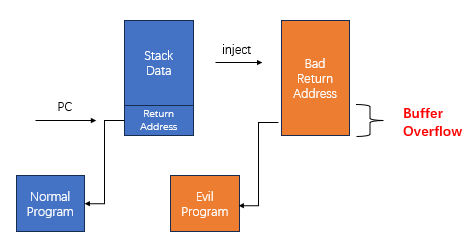
\includegraphics[width=0.5\textwidth]{pictures/Buffer Overflow.png}
  \caption{缓冲区溢出漏洞图示}
  \label{fig:BO}
\end{figure}
	
攻击者可能利用缓冲区溢出漏洞来执行恶意代码,例如注入Shellcode并强制程序跳转到
Shellcode的地址,从而获得系统权限。同时,也可能泄露敏感信息,例如通过溢出将重要
的内存区域覆盖为攻击者所控制的数据,从而导致信息泄露。除此之外,因为缓冲区溢出可
能导致程序崩溃或无法正常执行,使其无法提供正常的服务。

著名的``Code Red''蠕虫利用了Microsoft IIS服务器上的缓冲区溢出漏洞。攻击者通过发
送特制的HTTP请求,导致IIS的缓冲区溢出,并在受感染的系统上运行恶意代码。这导致系
统被感染并且在网络上传播蠕虫。
	
